\part{极限、连续}

\section{求数列极限}
数列极限的求解一般常用单调有界法、两边夹法、列紧性定理和柯西准则等等。下面对这几种常用方法进行总结。
\subsection{\texorpdfstring{$ \delta - \varepsilon  $}{δ-ε} 语言证明}
当需要证明$\lim_{n \to \infty} a_n = A$时,可以通过证明不等式$ \abs{a_n - A} < \varepsilon $成立。
\begin{situation}
    适用于给出数列递推公式的情况
\end{situation}
\paragraph{方法一} 直接对不等式证明:
\begin{proof}
    \[
        \forall \varepsilon > 0, ~ \exists N ~ \text{s.t. when}~ n > N,~
        \abs{a_n - A} < \varepsilon
    \]
\end{proof}


\paragraph{方法二} 对不等式进行缩放间接证明:
\begin{proof}
    由\[ \abs{a_n - A} \leq \varphi(n) < \varepsilon \]
    得出 \[ n > \psi(\varepsilon) \]
    不妨令 $N = \psi(\varepsilon)$,所以当 $n > N$时,恒有
    \[ \abs{a_n - A} < \varepsilon \]
    $\lim_{n \to \infty} a_n$存在
\end{proof}

\begin{example}
    设$ a > 1 $,证明$ \lim_{n \to \infty} \sqrt[n]{a} = 1 $
\end{example}
\begin{proof}
    根据几何不等式,得
    \[
        \abs{\sqrt[n]{a} - 1}
        = \sqrt[n]{a} - 1
        = (a \cdot \underbrace{1\cdots1}_{n-1})^{1/n} - 1
        < \frac{a+(n-1)}{n} - 1
        = \frac{a-1}{n}
    \]
    令$ \frac{a-1}{n}<\varepsilon $,即$ n > \frac{a-1}{\varepsilon} $。
    不妨令$N = \frac{a-1}{\varepsilon}$,则有
    \[
        \forall\varepsilon>0 \text{ and } n > N \qquad \abs{\sqrt[n]{a}-1} <\varepsilon
    \]
    所以$\lim_{n \to \infty} = 1$成立。
\end{proof}

\pagebreak
\subsection{单调有界法则}
单调有界法通常找出数列的上界(下界)。证明在趋于无穷时,数列单调增(单调减)。若有递推式,直接将递推式中的数列项换为极限值(未知数)进行求解。
\begin{theorem}
    \label{th:单调有界法则}
    单调有界数列必有极限
\end{theorem}
\begin{situation}
    适用于给出数列递推公式地情况
\end{situation}
\begin{example}
    设$a>0, x_1 > 0, x_{n+1} = \frac{1}{2}(x_n+\frac{a}{x_n}) (n=1,2,\cdots)$,求$\lim_{n\to\infty}x_n$
\end{example}
\begin{proof}
    由于
    \begin{alignat*}{2}
        x_{n+1}         & = \frac{1}{2}(x_n+\frac{a}{x_n}) & \geq  \sqrt{a} \\
        x_{n} - x_{n+1} & = \frac{1}{2x_n}(x_n^2-a)        & \geq  0
    \end{alignat*}
    所以$\{x_n\}$为单调有界数列,故可设$\lim_{n\to\infty} x_n = A$,当$n\to\infty$时,关系式
    \[ x_{n+1} = \frac{1}{2}(x_n+\frac{a}{x_n}) \]
    变为
    \[ A = \frac{1}{2}(A+\frac{a}{A}) \]
    解得$A=\sqrt{a}$,故$\lim_{n\to\infty} x_n =\sqrt{a}$
\end{proof}

\subsection{两边夹法则}
两边夹法则通常将数列左右两侧进行合适地缩放,两侧缩放得到地数列同时趋向同一个值时,则可以证明其极限存在。
\begin{theorem}
    \label{th:两边夹法则}
    (两边夹法则)若$n\to\infty$时,恒有
    \[ A \leftarrow x_n \leq y_n \leq z_n \rightarrow A \]
    或$\forall \varepsilon > 0, n\to\infty$
    \[ A -\varepsilon \leftarrow x_n(\varepsilon) \leq y_n \leq z_n(\varepsilon) \rightarrow A + \varepsilon \]
    则$\lim_{n \to\infty} y_n=A$
\end{theorem}
\begin{situation}
    已知数列通项
\end{situation}
\begin{example}
    证明$\lim_{n\to\infty}\sqrt[n]{n} = 1$
\end{example}
\begin{proof}
    根据平均不等式\ref{eq:平均不等式},有
    \[ 1 \leq \sqrt[n]{n} = (\underbrace{1\cdot 1\cdots 1}_{n-2}\sqrt{n}\cdot\sqrt{n})^{1/n}\leq \frac{n-2+2\sqrt{n}}{n} < 1+\frac{2}{\sqrt{n}} \to 1 \]
    由两边夹法则可知,$\lim_{n\to\infty}\sqrt[n]{n} = 1$
\end{proof}

\pagebreak
\subsection{柯西准则}
在极限值未知地情况下,判断数列极限的存在性可用柯西准则。
\begin{theorem}
    \label{th:柯西准则}
    (柯西准则)数列$\{x_n\}$收敛$\iff  \forall\varepsilon>0,\exists N,\text{ s.t. }m,n>N, \abs{x_m-x_n} <\varepsilon$
\end{theorem}
\begin{situation}
    只需判断极限是否存在
\end{situation}
\begin{example}
    证明数列$S_n=\sum_{k=1}^n \frac{1}{k}$发散
\end{example}
\begin{proof}
    因为
    \[ S_{2n} - S_{n} = \frac{1}{n+1}+\frac{1}{n+2}+\cdots+\frac{1}{n+n} \geq \frac{n}{2n} = \frac{1}{2}\]
    故${S_n}$发散。
\end{proof}

\subsection{运算法则}
如果数列由其它数列构成,且这些数列收敛,则可以通过运算法则,求出数列极限。
\begin{theorem}
    \label{th:数列极限运算法则}
    (运算性)设$\lim_{n\to\infty}x_n=A,\lim_{n\to\infty}y_n=B$,则有
    \begin{enumerate}
        \item $\lim_{n\to\infty} (x_n\pm y_n)=A\pm B$
        \item $\lim_{n\to\infty} x_ny_n=AB$
        \item $\lim_{n\to\infty} \frac{x_n}{y_n} = \frac{A}{B} \qquad (B\neq 0)$
    \end{enumerate}
\end{theorem}
\begin{situation}
    式子中含有收敛数列的组合(或者经过适当变形后),则可以通过运算法则求出极限
\end{situation}
\begin{example}
    求极限$\lim_{n\to\infty}\sqrt{n}(\sqrt{n-1}-\sqrt{n})$
\end{example}
\begin{solution}
    由于$\sqrt{n}$不存在,故不能直接用乘法法则,先经过适当变形
    \[
        \lim_{n\to\infty}   \sqrt{n}(\sqrt{n-1}-\sqrt{n})
        = \lim_{n\to\infty} \frac{\sqrt{n}}{\sqrt{n-1}+\sqrt{n}}
        = \lim_{n\to\infty} \frac{1}{1+\sqrt{1+\frac{1}{n}}}
        =\frac{1}{2}
    \]
\end{solution}

\begin{theorem}
    \label{th:数列极限保号性}
    (保号性)
    \[
        \text{If } \lim_{n\to\infty} x_n = A, \lim_{n\to\infty} y_n = B, A>B,
        \text{ s.t. } \exists N, n > N, x_n > y_n
    \]
\end{theorem}
\begin{theorem}
    \label{th:数列极限单调性}
    (单调性)
    \[
        \text{Let } \lim_{n\to\infty} x_n = A, \lim_{n\to\infty} y_n = B,
        \text{ if } x_n \geq y_n \text{ when } n\to\infty
        \text{ Hence } A \geq B
    \]
\end{theorem}
\begin{theorem}
    \label{th:数列极限子列性}
    (子列性)
    \[
        \lim_{n\to\infty} x_n = A \iff \lim_{n\to\infty} x_{k_n} = A \text{ for all sub array } \{x_{k_n}\} \text{ of } \{x_n\}
    \]
\end{theorem}

\subsection{Stolz定理}
类似与函数极限中的洛必达法则
\begin{theorem}
    \label{th:Stolz定理}
    若$\{y_n\}$\textcolor{red}{严格增无穷大},且有
    \[ \lim_{n\to\infty}\frac{x_n - x_{n-1}}{y_n - y_{n-1}} = A \]
    则有
    \[ \lim_{n\to\infty}\frac{x_n}{y_n} = A \]
\end{theorem}
\begin{situation}
    ~
    \begin{enumerate}
        \item 当数列通项中出现连加、连乘(指数对数化$x = \mathrm{e}^{\ln x}$将连乘转为连加)
        \item 当出现加减法的递推公式(即求\textcolor{red}{商差}的极限)时,可将问题转换为求解\textcolor{red}{商}的极限
    \end{enumerate}
\end{situation}
\begin{example}
    设$a_n>0 (n = 1, 2, \ldots) \lim_{n\to\infty}a_n = a$,证明$\lim_{n\to\infty}\sqrt[n]{a_1a_2\cdots a_n}=a$
\end{example}
\begin{proof}
    \[
        \lim_{n\to\infty} \sqrt[n]{a_1a_2\cdots a_n}
        =\exp(\lim_{n\to\infty}\frac{\ln a_1 + \cdots \ln a_n}{n})
        =\exp(\lim_{n\to\infty}\ln a_n) = \mathrm{e}^{\ln a} = a
    \]
\end{proof}
\begin{example}
    设$\lim_{n\to\infty}(x_n - x_{n-2}) = 0$,证明$\lim_{n\to\infty}\frac{x_n - x_{n-1}}{n} = 0$
\end{example}
\begin{proof}
    由于
    \[ \lim_{n\to\infty}\frac{x_{2n}}{2n} = \lim_{n\to\infty}\frac{x_{2n}-x_{2n-2}}{2n-(2n-2)} = 0 \]
    \[ \lim_{n\to\infty}\frac{x_{2n+1}}{2n+1} = \lim_{n\to\infty}\frac{x_{2n+1}-x_{2n-1}}{(2n+1)-(2n-1)} = 0 \]
    所以$\lim_{n\to\infty} \frac{x_n}{n} = 0$,从而
    \[ \lim_{n\to\infty}\frac{x_n - x_{n-1}}{n} = \lim_{n\to\infty}\frac{x_n}{n} - \lim_{n\to\infty}\frac{x_{n-1}}{n} = 0 \]
\end{proof}

\subsection{求和极限转积分}
根据积分的定义可以很容易知道如下公式
\[
    \int_{a}^{b} f(x) \dd{x} = (b-a)\lim_{n\to\infty}\frac{f(x_1) + f(x_2)+\cdots+f(x_n)}{n}\qquad x_i\in[a,b]
\]
此公式也可看做是$n$次蒙特卡洛积分后平均,其密度概率函数为$f_X(x)=\dfrac{1}{b-a}$
\[
    \int_a^b f(x) \dd{x} = \frac{1}{n}\sum_{i=1}^n \frac{f(x_i)}{\left.1\middle/(b-a)\right.}
\]
题目常常会出现求和极限的求解,此时可对原式变形后用积分求解。下式为常出现的情况:
\[
    \lim_{n\to\infty}\frac{1}{n}\left[f(\frac{1}{n}) + f(\frac{2}{n}) + \cdots + f(\frac{n}{n})\right] = \int_0^1 f(x) \dd{x}
\]


\section{函数极限}
\subsection{函数极限的概念}
由数列的极限类比,能得出如下定义
\begin{definition}
    \[ \lim_{x\to+\infty} f(x) = A \iff \forall\varepsilon >0, \exists X, \text{ 当~} x > X\text{ 时~}, \abs{f(x) - A} < \varepsilon \]
    \[ \lim_{x\to-\infty} f(x) = A \iff \forall\varepsilon >0, \exists X, \text{ 当~} x < X\text{ 时~}, \abs{f(x) - A} < \varepsilon \]
    \[ \lim_{x\to\infty}  f(x) = A \iff \forall\varepsilon >0, \exists X, \text{ 当~} \abs{x} > X\text{ 时~}, \abs{f(x) - A} < \varepsilon \]

    \[ \lim_{x\to x_0^+} f(x) = A \iff \forall\varepsilon > 0, \exists \delta > 0, \text{ 当~} 0 < x - x_0 < \delta \text{ 时~}, \abs{f(x) - A} < \varepsilon \]
    \[ \lim_{x\to x_0^-} f(x) = A \iff \forall\varepsilon > 0, \exists \delta > 0, \text{ 当~} 0 < x_0 - x < \delta \text{ 时~}, \abs{f(x) - A} < \varepsilon \]
    \[ \lim_{x\to x_0}   f(x) = A \iff \forall\varepsilon > 0, \exists \delta > 0, \text{ 当~} 0 < \abs{x-x_0} < \delta \text{ 时~}, \abs{f(x) - A} < \varepsilon \]

    \[  \lim_{x\to x_0}  f(x) = A \iff \lim_{n\to x_0^-} f(x) = \lim_{n\to x_0^+} f(x) = A \]

    \[ \lim_{x\to x_0} f(x) = \infty \iff \forall M, \exists \delta > 0, \text{ 使得~} 0 < \abs{x-x_0} < \delta \implies \abs{f(x)} > M \]
    \[ \lim_{x\to x_0} f(x) = +\infty \iff \forall M, \exists \delta > 0, \text{ 使得~} 0 < \abs{x-x_0} < \delta \implies f(x) > M \]
    \[ \lim_{x\to x_0} f(x) = -\infty \iff \forall M, \exists \delta > 0, \text{ 使得~} 0 < \abs{x-x_0} < \delta \implies f(x) < M \]
\end{definition}

\subsection{与数列极限的相似之处}
\begin{enumerate}
    \item 利用$\varepsilon-\delta$方式解函数的极限与数列的极限同理
    \item 运算法则相同
          \sidenote{
              对于有理函数$Q(x)$,即
              \[ Q(x) = \frac{a_0 + a_1x + \cdots + a_nx^n}{b_0 + b_1x + \cdots + b_mx^m} \]
              其中$a \neq 0, b \neq 0$,则有
              \begin{equation*}
                  \lim_{x\to\infty}Q(x) =
                  \begin{cases}
                      \frac{a_n}{b_m} & n=m \\
                      0               & n<m \\
                      \infty          & n>m
                  \end{cases}
              \end{equation*}
          }
    \item 局部保号性(\ref{th:数列极限保号性})
    \item 局部单调性(\ref{th:数列极限单调性})
    \item 两边夹法则(\ref{th:两边夹法则})
\end{enumerate}

\subsection{海涅定理}
当研究函数极限时,可以将函数转为数列进行极限的求解。
\begin{theorem}
    (海涅定理)
    \label{th:海涅定理}
    \[ \lim_{x\to x_0}f(x) = A \iff \forall x_n \to, \neq x_0, \text{ 都有~} \lim_{n\to\infty}f(x_n) = A \]
\end{theorem}
\begin{situation}
    证明极限不存在时,可以将函数$f(x)$转为研究$f(a_n)$和$f(b_n)$的极限,
    利用极限的唯一性可知,
    \begin{equation*}
        \lim_{x\to x_0}f(x) =
        \begin{cases}
            A             & \lim_{n\to\infty}f(a_n) = \lim_{n\to\infty}f(b_n) = A \\
            \text{不存在} & \lim_{n\to\infty}f(a_n) \neq \lim_{n\to\infty}f(b_n)
        \end{cases}
    \end{equation*}
\end{situation}
\begin{example}
    证明$\lim_{x\to 0}\sin\frac{1}{x}$不存在
\end{example}
\begin{proof}
    取$x_n=1/(2n\pi), y_n=1/(2n\pi + \pi/2)$则有
    \[ \lim_{n\to\infty}f(x_n) = 0 \neq 1 = \lim_{n\to\infty}f(y_n) \]
    根据海涅定理,$\lim_{x\to 0}\sin\frac{1}{x}$不存在。
\end{proof}

\subsection{变量代换(复合函数极限)}
当求解复合函数的极限时,外层函数极限转为内层函数极限。
\begin{theorem}
    \label{th:变量代换法则}
    (变量代换法则)
    \begin{enumerate}
        \item (去心法则)$\text{若~} x \to x_0\text{ 时~}, g(x)\to,\neq y_0, \text{ 则~}\lim_{y\to y_0}f(y)=A\text{ 时,}$
              \[ \lim_{x\to x_0} f(g(x)) = \lim_{y\to y_0} f(y) = A \]
        \item (连续法则)$\text{若~} \lim_{x\to x_0} g(x) = y_0 \text{ 且~} \lim_{y\to y_0} f(y) = f(y_0), \text{ 则,}$
              \[ \lim_{x\to x_0} f(g(x)) = f(\lim_{x\to x_0} g(x)) = f(y_0) \]
    \end{enumerate}
    注:去心和连续指的是$f(y)$在$y_0$处的连续性。
\end{theorem}

\subsection{等价公式}
等价公式在求解极限时,能很好地减少极限化简的计算量。
\begin{theorem}
    \label{th:等价公式}
    $\text{设~}x\to x_0\text{ 时~},\omega(x)\to,\neq 0, \text{则~}x\to x_0\text{ 时, 必有}$
    \begin{multicols}{2}
        \begin{enumerate}
            \item $\sin \omega(x) \sim \omega(x)$
            \item $\tan \omega(x) \sim \omega(x)$
            \item $\ln (1+\omega(x)) \sim \omega(x)$
            \item $\mathrm{e}^{\omega(x)}-1 \sim \omega(x)$
            \item $(1+\omega(x))^\alpha -1 \sim \alpha \omega(x) \qquad (\alpha \neq 0)$

            \item $1-\cos \omega(x) \sim \frac{1}{2}\omega^2(x)$
            \item $\omega(x)-\ln(1+\omega(x)) \sim \frac{1}{2}\omega^2(x)$
            \item $\mathrm{e}^{\omega(x)}-1-\omega(x) \sim \frac{1}{2}\omega^2(x)$

            \item $\tan \omega(x)-\omega(x) \sim \frac{1}{3}\omega^3(x)$
            \item $\omega(x)-\arctan \omega(x) \sim \frac{1}{3}\omega^3(x)$

            \item $\omega(x)-\sin \omega(x) \sim \frac{1}{6}\omega^3(x)$
            \item $\arcsin \omega(x) - \omega(x) \sim \frac{1}{6}\omega^3(x)$
            \item $\frac{\pi}{2} - \arccos \omega(x) - \omega(x) \sim \frac{1}{6}\omega^3(x)$

        \end{enumerate}
    \end{multicols}
\end{theorem}
\begin{situation}
    等价公式替换一般用于极限的\textcolor{red}{乘除过程}中。
    对于加减的极限,根据运算法则,\textcolor{red}{加减项必须的极限必须存在},才能进行替换(题中一般不会出现这种情况)。
    在使用等价公式时,通过对极限式子进行乘除调整,让其能消除某些项,从而达到简化的目的。


    \textbf{注:}此法本质时利用泰勒展开的第一项(一阶导数)进行计算,对于加减时,容易被消掉,故而对于加减的情况一般将其转为乘除形式。
\end{situation}

\begin{example}
    求极限$\lim_{x\to 0}\frac{1}{x^3}\left[ \left( \frac{2+\cos x}{3} \right)^x -1 \right] $
\end{example}
\begin{solution}
    \begin{align*}
          & \lim_{x\to 0}\frac{1}{x^3}\left[ \left( \frac{2+\cos x}{3} \right)^x -1 \right]    &                                                                 \\
        = & \lim_{x\to 0} \frac{1}{x^3}\left( \mathrm{e}^{x\ln\dfrac{2+\cos x}{3}} - 1 \right) & \qquad\text{替换~} \mathrm{e}^{\omega(x)}-1 \sim \omega(x)      \\
        = & \lim_{x\to 0} \frac{1}{x^3}\left( x\ln\dfrac{2+\cos x}{3} \right)                  &                                                                 \\
        = & \lim_{x\to 0} \frac{1}{x^2}\left[ \ln(1 + \dfrac{\cos x -1}{3})\right]             & \qquad\text{替换~} \ln(1+\omega(x)) \sim \omega(x)              \\
        = & \lim_{x\to 0} \frac{1}{x^2}\left( \dfrac{\cos x -1}{3} \right )                    & \qquad\text{替换~} 1-\cos \omega(x) \sim \frac{1}{2}\omega^2(x) \\
        = & \lim_{x\to 0} \frac{1}{x^2}\left( -\frac{1}{6}x^2 \right)                          &                                                                 \\
        = & -\frac{1}{6}
    \end{align*}
\end{solution}

\subsection{洛必达法则}
洛必达法则可以将用代入方法计算的极限转化为导数商的极限,从而解决复杂的极限计算。
\begin{theorem}
    \label{th:洛必达法则}
    (洛必达法则)
    ~
    \begin{enumerate}
        \item $\text{设~}x\to x_0\text{ 时}, f(x),g(x)\text{ 是无穷小且~}g'(x)\neq 0,$
        \item $\text{设~}x\to x_0\text{ 时}, g(x)\text{ 是无穷大且~}g'(x)\neq 0,$
    \end{enumerate}
    \[ \text{若~}\lim_{x\to x_0}\frac{f'(x)}{g'(x)}=A, \text{ 则~} \lim_{x\to x_0}\frac{f(x)}{g(x)}=A \]
\end{theorem}
\begin{situation}
    在使用洛必达法则时,应尽量先尝试直接代入计算,再用等价公式进行变形化简,最后才使用洛必达,这样能减少不必要的求导计算。
\end{situation}
\begin{example}
    $\text{设~}y=\left(\frac{\pi}{2}-\arctan x\right)^{\frac{1}{\ln x}}, \text{ 求~}\lim_{x\to +\infty}y$
\end{example}
\begin{solution}
    \begin{align*}
        \lim_{x\to +\infty}\ln y
         & = \lim_{x\to +\infty}\frac{\ln\left(\frac{\pi}{2}-\arctan x\right)}{\ln x}                                     \\
         & = \lim_{x\to +\infty}\left. \frac{-1}{(1+x^2)\left(\frac{\pi}{2}-\arctan x\right)} \middle/ \frac{1}{x}\right. \\
         & = \lim_{x\to +\infty} \frac{-1/x}{\frac{\pi}{2}-\arctan x}                                                     \\
         & = \lim_{x\to +\infty} \frac{1/x^2}{-\frac{1}{1+x^2}} = -\lim_{x\to +\infty} \left(1+\frac{1}{x^2}\right)       \\
         & =-1
    \end{align*}
    所以 $\lim_{x\to +\infty}y=\mathrm{e}^{-1}$
\end{solution}

\subsection{泰勒公式}
泰勒公式求极限属于万金油的方法。
\begin{theorem}
    \label{th:泰勒公式}
    (泰勒公式)
    设函数$f(x)$在$x_0$点的邻域$(a,b)$内有$n+1$阶导数,则对$\forall x\in (a,b)$,都有介于$x_0$和$x$之间的$\xi$,使得
    \begin{multline*}
        f(x) = f(x_0) + f'(x_0)(x-x_0) + \frac{f''(x_0)}{2!}(x-x_0)^2+\cdots\\
        +\frac{f^{(n)}(x_0)}{n!}(x-x_0)^n+\frac{f^{n+1}(\xi)}{(n+1)!}(x-x_0)^{n+1}
    \end{multline*}
\end{theorem}
\begin{situation}
    对极限中的复杂项展开至相同阶数,化简后进行求解
\end{situation}
\begin{example}
    求\[ \lim_{x\to +\infty}\left[x-x^2\ln\left(1+\frac{1}{x}\right)\right] \]
\end{example}
\begin{solution}
    \[
        \lim_{x\to +\infty}\left[x-x^2\ln\left(1+\frac{1}{x}\right)\right]
        = \lim_{x\to +\infty}\left[x-x^2\left(\frac{1}{x}-\frac{1}{2x^2}\right)\right]
        = \lim_{x\to +\infty}(x-x+\frac{1}{2})
        =\frac{1}{2}
    \]
\end{solution}

\section{函数的连续性}
\subsection{连续性}
函数的连续性考察,常常出现于选择题中。故对函数连续的基本概念要牢牢掌握。
\begin{definition}
    (连续性)
    \begin{alignat*}{4}
         & \lim_{x\to x_0^-}f(x) & ~ = f(x_0) & = \lim_{x\to x_0^+}f(x) & \text{ (连续)}   \\
         & \lim_{x\to x_0^-}f(x) & ~ = f(x_0) &                         & \text{ (左连续)} \\
         &                       & ~ f(x_0)   & = \lim_{x\to x_0^+}f(x) & \text{ (右连续)}
    \end{alignat*}
    当任何一项不存在或等号不成立时,则函数在$x_0$不连续(左不连续、右不连续)。
\end{definition}

\begin{theorem}
    \label{th:连续函数运算性}
    (运算性)
    设函数$f(x),g(x)$在$x_0$处连续,则函数$f(x)\pm g(x), f(x)g(x), \frac{f(x)}{g(x)} (g(x)\neq 0)$在$x_0$处连续
    \\
    若$g(u)$在$u=f(x_0)$处连续,则复合函数$g\circ f(x)$在$x_0$处连续
\end{theorem}

\subsection{间断点}
当讨论函数的间断点时,具体步骤如下:
\begin{enumerate}
    \item 考虑其定义域,找到其间断点
    \item 计算间断点的左右极限,(间断点可能有定义)
    \item 根据间断点的左右极限,判断间断点的类型
\end{enumerate}
\begin{definition}
    (间断点)函数$f(x)$在$x_0$处不连续,则称$x_0$为函数$f(x)$的间断点\\
    \begin{math}
        \begin{cases}
            \text{第一类间断点}
            \begin{cases}
                \text{可去间断点}\qquad (\text{左右极限相等}) \\
                \text{跳跃间断点}\qquad (\text{左右极限不等})
            \end{cases}
            \qquad (\text{左右极限存在})
            \\
            \text{第二类间断点}
            \begin{cases}
                \text{无穷间断点}\qquad (\text{无穷大}\frac{1}{x}) \\
                \text{振荡间断点}\qquad (\text{振荡}\sin\frac{1}{x})
            \end{cases}
            \qquad (\text{左极限或右极限不存在})
        \end{cases}
    \end{math}
\end{definition}
\begin{marginfigure}
    \centering
    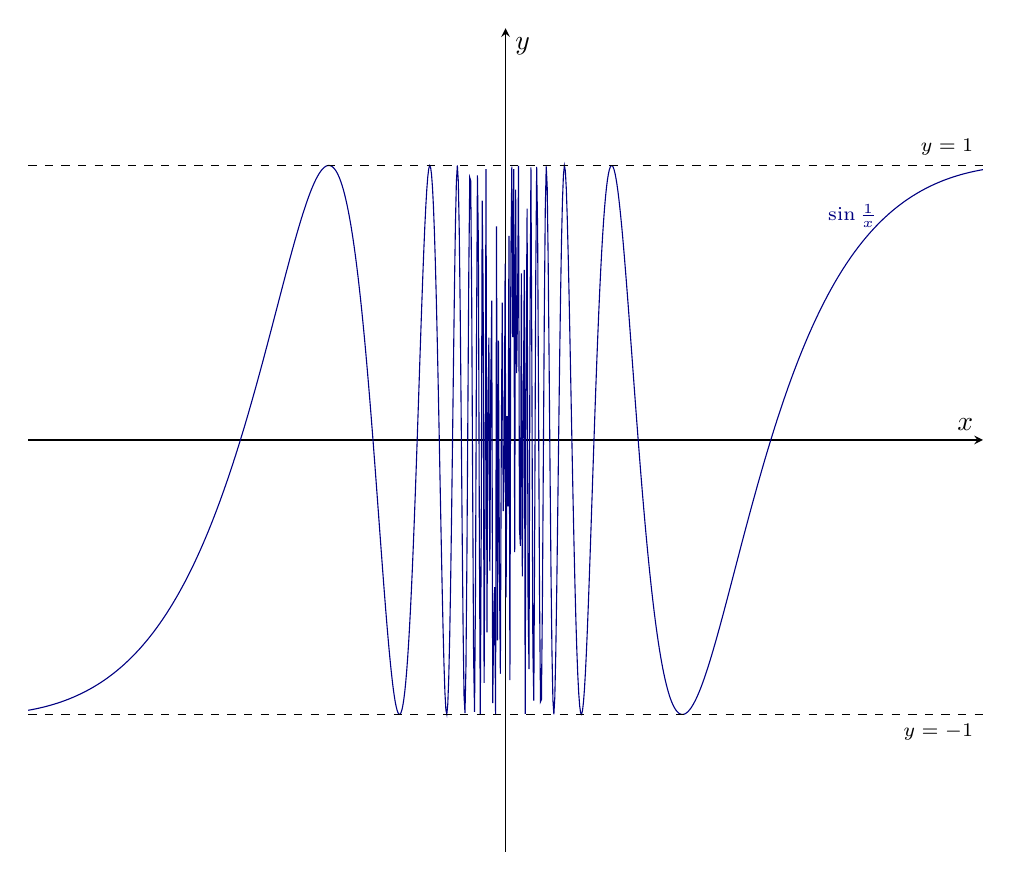
\begin{tikzpicture}
        \begin{axis}[
                ticks=none,
                axis lines=middle,
                ymin=-1.5,
                ymax=1.5,
                domain=-0.01:0.01,
                xlabel=$x$,
                ylabel=$y$,
                scale only axis,
                width=\textwidth
            ]
            \addplot[NavyBlue,samples=1000] {sin(1/x)} node[pos=0.998,left]{\scriptsize$\sin\frac{1}{x}$};
            \addplot[dashed]{1}  node[above left]{\scriptsize$y=1$};
            \addplot[dashed]{-1} node[below left]{\scriptsize$y=-1$};
        \end{axis}
    \end{tikzpicture}
    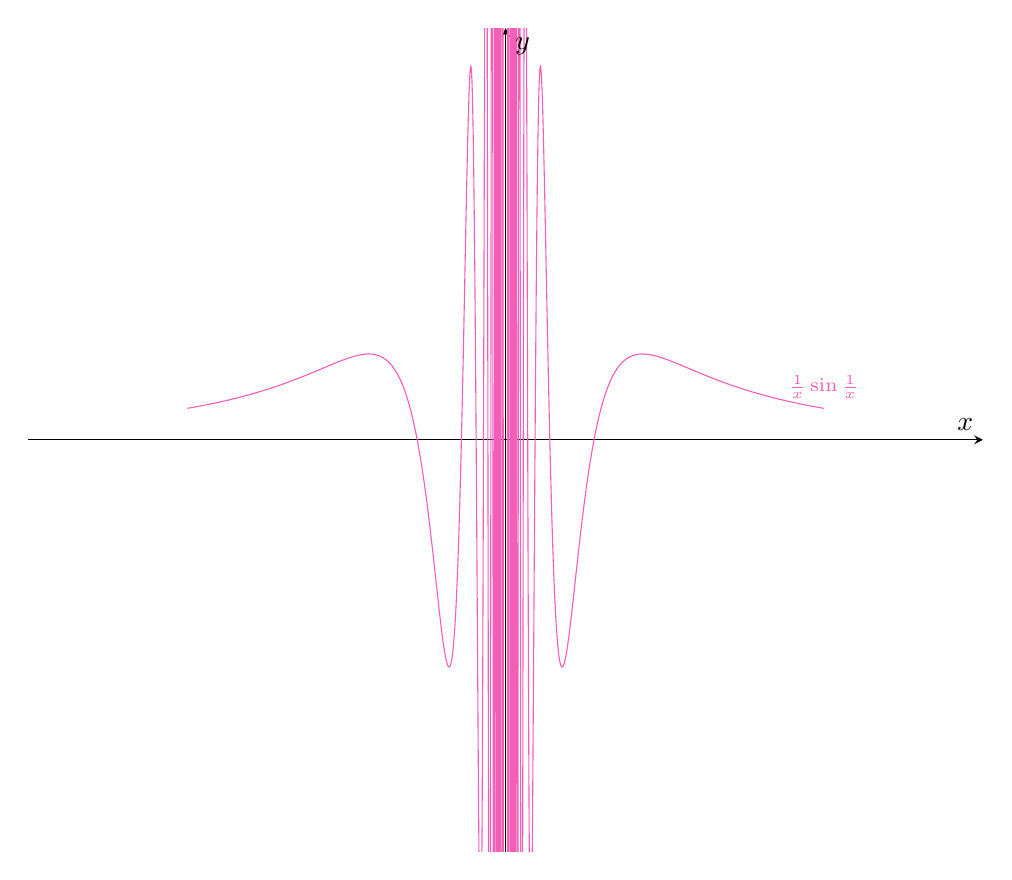
\begin{tikzpicture}
        \begin{axis}[
                ticks=none,
                axis lines=middle,
                ymin=-500,
                ymax=500,
                xmin=-0.03,
                xmax=0.03,
                xlabel=$x$,
                ylabel=$y$,
                scale only axis,
                width=\textwidth
            ]
            \addplot[CarnationPink,domain=-0.02:-0.0001,samples=1000] {sin(1/x)/x};
            \addplot[CarnationPink,domain=0.0001:0.02,samples=1000] {sin(1/x)/x} node[above]{\scriptsize$\frac{1}{x}\sin\frac{1}{x}$};
        \end{axis}
    \end{tikzpicture}
    \caption{有界振荡和无界振荡}
\end{marginfigure}
间断点不是无穷大则说明了,此间断点左右极限存在,或振荡(可有界如$\sin \frac{1}{x}$在$x=0$处,或无界如$\frac{1}{x}\sin \frac{1}{x}$)


\subsection{一致连续}
.
\begin{definition}
    \label{def:一致连续}
    (一致连续)
    $\forall \varepsilon>0,\exists \delta>0, \text{ 当~}x,y\in I \text{ 且~} \abs{x-y}< \delta \text{ 时,恒有}$
    \[ \abs{f(x)-f(y)} <\varepsilon \]
\end{definition}
\begin{theorem}
    若函数$f(x)$的一阶导数$f'(x)$有界,则函数$f(x)$一致连续。(可通过中值定理得证)
\end{theorem}
\begin{proof}
    因为$\abs{f'(x)} < M$,根据中值定理,对于定义域内任意的$a,b,\abs{a-b} < \delta$,令$\delta=\frac{\varepsilon}{M}$可得
    \[
        \abs{f(a) - f(b)}
        = \abs{f'(\xi)(a-b)}
        < M\abs{a-b}
        < M\delta = \varepsilon
    \]
\end{proof}

\subsection{闭区间上连续函数的性质}
此性质的考察通常出现与选择题、证明题中。
\begin{theorem}
    (有界性定理)闭区间上的连续函数一定是有界函数
\end{theorem}
\begin{theorem}
    (最值定理)闭区间上的连续函数一定有最大值和最小值
\end{theorem}
\begin{theorem}
    (介值定理)若$C$介于$f(a),f(b)$,则一定有$f(\xi)=C \qquad (\xi\in[a,b])$
\end{theorem}
\begin{theorem}
    (零点定理)若闭区间$[a,b]$上的连续函数$f(x)$,有$f(a)f(b)<0$则一定有$f(\xi)=0 \qquad (\xi\in(a,b))$
\end{theorem}
\begin{theorem}
    (一致连续定理)闭区间上的连续函数必一致连续\ref{def:一致连续}
\end{theorem}

